% This paper is copyright 2021 the authors.

% people who might comment on it:
% -------------------------------
% - KSF
% - Kilian Walsh
% - Sanjoy Mahajan
% - David Grier
% - All those in the acks.

% style notes:
% ------------
% - Always air before water, always sail before keel before hull.
% - Need to choose typesetting for GoodSailing and BetterSailing and then be consistent.
% - Maybe the "flat" force should be the "planar" force?

% to-do items:
% ------------
% - Add to the abstract the point that the sailboat is defined by 3 dimensionless numbers: The sail-to-keel ratio, and two lift ratios.
% - confirm that "lift ratio" is the correct terminology.
% - Switch to calling the sail and keel orientations "effective orientations" not just orientations. And say why.
% - make sure I clearly introduce the concept of lift ratio and stick with it.
% - Change citations to Tao to make it clear that the Tao model is (probably) wrong!!
% - Make sure I cite {symmetry} appropriately in various places. Probably also point out that it is a fun longer read.
% - Make sure we aren't claiming that the model is NOVEL. It is just SIMPLE.
% - Reconsider the post-equation commas? (HWR SAY).
% — Make some comments on the situations in which the ram-pressure force approximation is more appropriate---gale force or lull?
% - Is the latex footnote-footnote separation fucked?
% - Do we still mention "tensors" anywhere? make sure the abstract is consistent with the body.
% - What claims in the literature exist about maximum boat speeds? Have I seen a 2x wind claim? We can beat that. Have I seen a "never faster downwind than the wind" (as in Kimball) or than 0.5 times the wind claim? We can beat that too.
% - Respond to comments by Hyung Don Ryoo, in email to Hogg, 2021-07-15.
% - Make sure the spirit of the bibliographic comments get pulled into the main text.
% - Somewhere comment that the wind is a function of height, which means that another approximation has to do with what particular mean wind speed we are considering.
% - Are we clear that we also find that you can sail faster than the wind, in general, like cross-wind? Emphasize that when we first figure it out.
% - Need to pull in most recent figures; parameters have changed.

\documentclass[letterpaper]{article}
\usepackage[utf8]{inputenc}
\usepackage[letterpaper]{geometry} % because Overleaf is weird.
\PassOptionsToPackage{hyphens}{url}\usepackage{hyperref}
\usepackage{graphicx}
\graphicspath{{./}{../ipynb/}}

% math macros
\usepackage{amsmath, amsfonts}
\DeclareMathOperator*{\argmax}{argmax}
\newcommand{\dd}{\mathrm{d}}
\renewcommand{\vec}[1]{\boldsymbol{#1}}
\newcommand{\uvec}{\vec{\hat{e}}}
\newcommand{\tensor}[1]{\mathbb{#1}}
\renewcommand{\flat}{\text{flat}}
\newcommand{\iso}{\text{iso}}
\newcommand{\air}{\text{air}}
\newcommand{\water}{\text{water}}
\newcommand{\boat}{\text{boat}}
\newcommand{\destination}{\text{dest}}
\newcommand{\good}{\text{(good)}}
\newcommand{\better}{\text{(better)}}
\newcommand{\sail}{\text{sail}}
\newcommand{\keel}{\text{keel}}
\newcommand{\hull}{\text{hull}}
\renewcommand{\above}{\text{above}}
\newcommand{\below}{\text{below}}
\newcommand{\vair}{\vec{v}_\air}
\newcommand{\vwater}{\vec{v}_\water}
\newcommand{\vboat}{\vec{v}_\boat}
\newcommand{\vdest}{\vec{v}_\destination}
\newcommand{\mm}{\mathrm{m^2}}
\newcommand{\mps}{\mathrm{m\,s^{-1}}}
\newcommand{\mmps}{\mathrm{m^2\,s^{-1}}}

% text macros
\newcommand{\documentname}{\textsl{Article}}
\newcommand{\secref}[1]{Section~\ref{#1}}
\newcommand{\figref}[1]{Figure~\ref{#1}}

% typesetting adjustments
\makeatletter
\renewcommand\section{\@startsection {section}{1}{\z@}%
  {-3.25ex \@plus -1ex \@minus -.2ex}%
  {1.5ex \@plus .2ex}%
  {\raggedright\normalfont\large\bfseries}}
\makeatother
\setlength{\textwidth}{5.00in}
\setlength{\oddsidemargin}{3.25in}
\addtolength{\oddsidemargin}{-0.5\textwidth}
\setlength{\textheight}{9.00in}
\setlength{\topmargin}{-0.40in}
\pagestyle{myheadings}
\newcommand{\figurerule}{\rule[1ex]{\textwidth}{0.2pt}}
\linespread{1.08}
\frenchspacing\sloppy\sloppypar\raggedbottom

\title{\bfseries%
A simple momentum-transport model for sailing}
\markright{\textsf{Hogg \& Kleban / Momentum-transport model for sailing}}
\author{DWH, MK, others?}
\date{2021}
\begin{document}
\maketitle

\begin{abstract}\noindent
    We present a simplified model for the forces on a sailboat.
    Our model is that there is a ram-pressure force on the sail, with a magnitude and direction that depend on the relative air--boat velocity and the sail orientation.
    Similarly, there is a ram-pressure force on the keel, depending on the relative water--boat velocity and the keel orientation.
    The resulting expression for the total force on the boat is coordinate-free and consistent with Galilean relativity.
    The solutions corresponding to sailing in steady wind correspond to boat velocities that deliver vanishing total force, given the angles of the sail and keel.
    We use this simple model to derive simple properties of sailing that are not far off from standard folklore and measurements.
    One consequence of this model is that a sailboat does not move (relative to the water) precisely in the direction that its keel points (the direction of the prow); it moves slightly downwind of that.
    Another consequence is that it is possible for an extremely well designed boat (very good lift ratios) to sail downwind (relative to the water) \emph{faster than the wind}, on a tacking course.
    Another is that cross-wind sailing is fastest when the effective area of the sail is larger than the effective area of the keel by the ratio of the density of water to the density of air.
    Nothing conceptual about this model depends on the \emph{curvature} of the sail, in contradiction to some folk explanations of sailing; the important thing is that the model \emph{does} depend on angular re-direction of fluid momentum flux; sail curvature can help with this.
\end{abstract}

\section{Introduction}\label{sec:intro}

We (the authors) are not sailors!
However, we believe that sailing is a beautiful technology.
The boat is powered by the wind, and yet it can travel (possibly with a tacking course) in any direction.
Of course it's not consistent with Galilean relativity\footnote{We refer to Galilean relativity repeatedly in this \documentname.
Of course Galilean relativity is just the low-velocity approximation to special relativity \cite{sr}.
But we are not going to consider air--water velocity differences that are an appreciable fraction of the speed of light (except maybe in the discussion in \secref{sec:discussion}).} to say that the boat is powered by the wind:
There is no absolute velocity, and there is a valid rest frame in which the wind velocity is zero.
The Galilean-relativistic thing to say is that the boat is powered by the relative velocity between the air and the water.
Indeed, the symmetry between the air and the water in the mechanisms of sailing is the fundamental theme of one of the better books on the physics of sailing \cite{symmetry}.
Here we build the simplest possible physical model for a sailboat---and sailing---that is consistent with symmetries and captures all of the leading-order features of the technology.

KLEBAN: Write things about ddwfttw, maybe? For context only! But it is worth saying that if we can understand sailing with a simple model, we might resolve some disputes about ddwfttw.

When we were little, we were taught a story about how airfoils (wings on airplanes, for example) generate lift, in which the air path over the top of the lenticular, curved wing is longer than the path under the bottom, so velocities are different (top to bottom), and thus there is a net force from a difference in Bernoulli pressures.
This model is now known to be wrong (see, for example, \cite{lift}):
There is no reason for the air flow to ``join up'' at the end of the airfoil.
And, besides, airplanes can fly upside-down!
The best leading-order description is that the lift on the wing comes from \emph{redirection of the flow of air}.
There is a volumetric rate of momentum change downwards in the air flowing onto the wing, which leads to an equal-and-opposite force upwards on the wing.
Similarly, the force on a sailboat sail is from the redirection of the flow of the air encountering the sail.
This point is made admirably in some books on the physics of sailing (especially \cite{sails}).
And the force on a sailboat keel is from the redirection of the flow of water encountering the keel.
These forces are sometimes called ``lift'' forces in analogy to the lift force on an airplane wing.
This \documentname{} is partially motivated by these observations.
Sailboats sail by managing momentum changes in the air and water.
They work on \emph{momentum transport}.

There are multiple books about the physics of sailing (including \cite{symmetry, explained, sails, pos}).
These books vary in their physical correctness and their comprehensiveness.
They are mainly aimed at sailors who want to understand better their boats and how to design them and sail them.
This paper is aimed at physicists and students of physics interested in a simple, implementable, physically justifiable model of sailing.
This model is a sandbox for experimenting with wind-powered travel and wind-powered machines, which are, in turn, key concepts in sustainable technology.
Our model of sailing is also something that can be implemented by students new to physics, in extremely simple code (an example of which is released in conjunction with this \documentname\footnote{All code used in this \documentname{} is available under a HOGG WHAT LICENSE? at \url{https://github.com/davidwhogg/Sailing}.}).

Importantly in what follows, we deliver only zeroth-order physical explanations.
In detail, the flow of air over a sail, and water over a keel, involves boundary layers, turbulence, and all the subtleties and complexities of fluid dynamics.
We drop all of that in favor of a pure-momentum model that erases all of these critical details, and boils all of this down to some effective areas and direction vectors.
This over-simplification might be frustrating to sailing experts, or fluid dynamicists.
But our goal is to find the simplest possible, dimensionally correct, Galilean-relativistic rules for a boat that can sail non-trivially.
You might say that this is an astrophysics-quality model of a sailboat!
The only prior work we know in this space is \cite{tao}, but that model is (in our view) overly simplistic, and maybe dimensionally incorrect (it appears to make forces proportional to velocities, instead of squared velocities).
In principle also \cite{pos} delivers similar equations to what we derive below, based on similar considerations and similar approximations, but their goals are not really for their reader to build an implementable model.

Above, we've mentioned Galilean relativity:
It is important that any model for a sailboat precisely obey Galilean relativity; it is an extremely important symmetry for understanding sailing \cite{symmetry}.
Indeed---according to lore---Galilean relativity was discovered by consideration of doing physics experiments in the hold of a sailing ship \cite{galileo}.
The contemporary view of Galilean relativity is that all velocities that appear in physical law or the prediction of observables must be relative velocities.
In addition to obeying this symmetry, our model is consistent with dimensional analysis and is equivariant to rotations and reflections.
We also make use of good, coordinate-free expressions.

Our model for forces on a sailboat presented below in \secref{sec:model} is a very generic momentum-transport model.
In astrophysics contexts, forces from momentum transport from winds or relative motions of bodies and fluids are called ``ram-pressure'' forces.
We use that term a bit in what follows, but since it means different things to different people, it's fine to substitute in the word ``lift'' for ``ram-pressure'' everywhere.
We'll discuss these forces conceptually in \secref{sec:ram}, give Galilean-relativistic expressions in \secref{sec:model}, and use them to explain the steady-state motion of a sailboat in \secref{sec:steady}.
We follow this modeling with some optimization, useful to an idealized sailor on our idealized boat, in \secref{sec:good} and \secref{sec:better}.
When we optimize the trim of our boat, we learn about what things the boat can do, in terms of sailing speed, and sailing upwind and downwind.
It's impressive!
We will discuss the dependence of our results on our boat properties in \secref{sec:design}.
We comment on the implementation of the model in \secref{sec:implementation} and we remark on limitations and extensions in \secref{sec:discussion}.

\section{Why ram-pressure forces?}\label{sec:ram}

Sailboats and sails---like airplanes and wings---are beautiful curved structures that are designed to redirect air with as little turbulence as possible.
So why would we make a planar-sail approximation and model that planar sail with a ram-pressure force?
Ram-pressure forces are generally associated with bow shocks and turbulent wakes.
Many things (cars, launch vehicles) are designed to \emph{avoid} the ram-pressure effect known as air resistance or drag.

Fundamentally, a sailboat sail works by redirecting the momentum of the air.
%, in the rest frame of the boat.
%It does that in every frame!
More specifically, there is a momentum flux (momentum per unit time) that intersects the sail (and some neighborhood around the sail).
The air that intersects the sail and neighborhood gets redirected, and so there is  a rate of momentum change on the air due to the sail.
%in direction.
%There is therefore not just a momentum flux into the sail, there is a rate of momentum change being input into the air from the sail.
That momentum transport---the (vector) change in momentum in the air per unit time---is the (vector) force on the air from the sail.
Half of the explanation for how a sailboat sails uses the equal-and-opposite reaction to this force (the other half of the explanation will come from the keel).

This momentum-transport explanation of a sail (or a wing) 
%has an expression that is, essentially,
can be expressed as a particle flux (number per time) times a change in momentum per particle.
These are also the physical components of a ram-pressure force.
Indeed, the most basic derivation of the ram-pressure force is in the microscopic model of an ideal gas, in which particles bounce elastically off the surface, changing their momenta.
HOGG PUT A DIAGRAM HERE AND EQUATIONS.
In this ideal-gas model, the mean force on the surface can be thought of as the combination of many tiny impulses per unit time from these elastic collisions.
What's important about the model, however, is the momentum transport:
The incoming momentum flux upstream of the surface is different than the outgoing momentum flux downstream of the surface.
%The force on the sail can be thought of as being generated by the vector change in that momentum flux.
%A bit repetitive, possibly trim more

In this paper we are not arguing that ram pressure on flat sails is a complete explanation of a sailboat!
We are arguing that the sailboat can be modeled as having two important surfaces---the sail and the keel---one of which deviates the flow of air, and the other deviates the flow of water.
The angles of the sail and keel with respect to the air--boat and water-boat velocity vectors set the angular deviations of the two fluids, and therefore both the magnitudes and the directions of the sail and keel forces.
The directions of the forces can be manipulated to create amazing boat dynamics and kinematics.
The point of this \documentname{} is that much of the amazing dynamics can be understood in an amazingly simple model for the sailboat.
So while we use the phrases ``flat sail'' and ``ram-pressure'' in what follows to describe our model, we really mean ``simple momentum transport''.

\section{Ram-pressure sailboat}\label{sec:model}

We are going to work in 2D (you can think of the two dimensions as the surface of a map of a local patch of the Earth, if you like), with velocities $\vec{v}$ and forces $\vec{F}$ that are column vectors (or $2\times 1$ matrices).
To stay coordinate-free, we are going to talk about angles as orientations of unit vectors like $\uvec_{\perp\sail}$ and $\uvec_{\parallel\sail}$ (which will be defined below).
If you prefer to think in terms of angles, you can choose a coordinate system and then
\begin{align}
    \uvec_{\perp\sail} &= \begin{bmatrix}\cos\theta_\sail \\ \sin\theta_\sail\end{bmatrix} ~ ; ~ \uvec_{\parallel\sail} = \begin{bmatrix}-\sin\theta_\sail \\ \cos\theta_\sail\end{bmatrix} ~,
\end{align}
for some angle $\theta_\sail$ in that coordinate system.
We won't particularly use angles much in what follows, but if you want to come back to angles, you can take the arctangent of the components of $\uvec_{\perp\sail}$.

Our sailboat is going to be a simple anisotropic object such that wind that hits its planar sail produces a ram-pressure force perpendicular to the surface of the sail,
and water that hits its planar keel produces a ram-pressure force perpendicular to the surface of the keel.
We can construct the complete force law on the sailboat by thinking about ram-pressure forces on surfaces.
As we note above, if the fluid (air or water in this case) is thought of as being composed of particles that bounce elastically off of a flat surface of area $A$, then the ram-pressure force on that surface is
\begin{align}\label{eq:flat}
    \vec{F}_\flat &= \eta\,\rho\,A\,(\uvec_\perp\cdot\vec{v})^2\,\uvec_\perp ~,
\end{align}
where $\eta$ is a dimensionless prefactor, $\rho$ is the density of the fluid, $\uvec_\perp$ is the unit vector perpendicular to the surface (oriented such that it points down-flow), $\vec{v}$ is the %velocity of the fluid in the rest frame of the surface, 
relative velocity between the fluid and the surface,
and $\uvec_\perp\cdot\vec{v}$ is the scalar inner product (dot product) of the two vectors.

Na\"ively in the particle-collision model the prefactor $\eta$ is 2, but in the world of real fluids it depends on the shape of the surface, the velocity, and (if things are tiny) the viscosity.\footnote{%
Viscosities only matter for very small objects, much smaller than sailboats. The way to see this is by computing the Reynolds number, which, loosely speaking, is the ratio of inertial forces to viscous forces. It is a typical lengthscale (like the height of the sail) times a typical velocity (like the relative velocity of the boat and air) divided by the kinematic viscosity (something like $10^{-5}\,\mmps$ for air and $10^{-6}\,\mmps$ for water). Typical Reynolds numbers for both the boat--air contact and the boat--water contact are therefore on the order of $10^6$ to $10^7$ for real boats in typical conditions. That is, viscosity plays no first-order role in sailing. In detail it shapes the turbulence in the wakes coming off the sail and keel edges, but that is a tiny detail from perspective of our brutal model.}
We're going to treat $\eta$ as an uninteresting constant; in particular we are going to assume that it doesn't depend on velocity, such that it can be combined with the area $A$ (to make an effective area) in everything that follows.
If you don't like that we had to orient the unit vector $\uvec_\perp$ ``down-flow'', then you can manage the signs by re-writing \eqref{eq:flat} as
\begin{align}\label{eq:flat2}
    \vec{F}_\flat &= \eta\,\rho\,A\,|\uvec_\perp\cdot\vec{v}|\,(\uvec_\perp\cdot\vec{v})\,\uvec_\perp ~;
\end{align}
in this formulation, $\uvec_\perp$ can point in either of the two directions that are normal to the surface.
The force law \eqref{eq:flat} and \eqref{eq:flat2} is very similar to what's derived or discussed in \cite{symmetry} (Section~8.4) and in \cite{pos} (Chapters~2, 3).

If, instead of a planar object, you have an isotropic object (a sphere in fully 3D situations, an axisymmetric boat in our 2D water world), the ram-pressure force becomes
\begin{align}\label{eq:iso}
    \vec{F}_\iso &= \eta\,\rho\,A\,|\vec{v}|\,\vec{v}
\end{align}
where $\eta$ is a (different) dimensionless prefactor, $A$ is now the cross-sectional or projected area of the surface, and $\vec{v}$ is still the fluid velocity in the rest frame of the object.
Again $\eta$ depends on velocity, but again we are going to ignore that.

Our model for a sailboat is going to be that it is a composite object, composed of a flat sail, a flat keel, and an isotropic partially submerged hull.
Thus the ram-pressure force on the sailboat will have four components, a force on the flat sail from the air, a force on the flat keel from the water, a force on the hull from the air, and a force on the hull from the water.
This model is extremely simplistic!
In some sense it is the closest possible object to the spherical cow that will sail non-trivially.
In detail the forces from the air are given by
\begin{align}\label{eq:startmodel}
  \vec{F}_\air &= \vec{F}_{\sail-\air} + \vec{F}_{\hull-\air}
  \\
  \vec{\Delta v}_\air &\equiv \vair - \vboat \label{eq:deltav}
  \\
  \vec{F}_{\sail-\air} & = \rho_\air\,A_\sail\,(\uvec_{\perp\sail}\cdot\vec{\Delta v}_\air)^2\,\uvec_{\perp\sail} \label{eq:Fsailair}
  \\
  \vec{F}_{\hull-\air} & = \rho_\air\,A_{\above}\,|\vec{\Delta v}_\air|\,\vec{\Delta v}_\air \label{eq:Fhullair} ~,
\end{align}
where we have dropped the $\eta$ prefactors (or really combined them with the area constants, to make the area constants \emph{effective areas}), $\vair,\vboat$ are the velocities of the air and boat, $A_\sail$ is an effective area related to the area of the sail, $\uvec_{\perp\sail}$ is a unit vector perpendicular to the plane of the planar sail, and $A_{\above}$ is an effective area related to the area of the boat's hull that is above the water surface.
Similarly, the forces from the water are given by
\begin{align}
  \vec{F}_\water &= \vec{F}_{\keel-\water} + \vec{F}_{\hull-\water}
  \\
  \vec{\Delta v}_\water &\equiv \vwater - \vboat
  \\
  \vec{F}_{\keel-\water} & = \rho_\water\,A_\keel\,(\uvec_{\perp\keel}\cdot\vec{\Delta v}_\water)^2\,\uvec_{\perp\keel}
  \\
  \vec{F}_{\hull-\water} & = \rho_\water\,A_{\below}\,|\vec{\Delta v}_\water|\,\vec{\Delta v}_\water ~,\label{eq:endmodel}
\end{align}
where the sail is replaced by the keel everywhere, and $A_{\below}$ is an effective area related to the area of the hull below the water surface.

In some of what follows, we will make use of dimensionless ratios of effective areas.
For example, the ratio of sail to keel $A_\sail/A_\keel$ will affect the ratio of upwind to downwind sailing speeds (and, surprisingly, affect cross-wind sailing).
For another, the ratios of sail and keel to the relevant parts of the hull $A_\sail/A_\above$ and $A_\keel/A_\below$ act like ``lift ratios'' in the study of flying:
They control the ratio of useful sailing forces to drag.
We will refer to these---na\"ively---as lift ratios in what follows.

The above model could be called ``isotropic boat, thin planar sail and keel''.
There is an alternative model to be made, using the same elements, which could be called ``parallelepiped sail, parallelepiped keel''.
This alternative model uses only the flat-plane force law \eqref{eq:flat}, but the sail and keel each are treated as parallelepipeds with large areas $A_\sail$ and $A_\keel$ and then much smaller perpendicular areas $A_{\sail\parallel}$ and $A_{\keel\parallel}$.
So, for example, the force from the air on the boat in this model is
\begin{align}
  \vec{F}_\air &= \vec{F}_{\sail-\air} + \vec{F}_{\parallel-\air}
  \\
  \vec{F}_{\parallel-\air} & = \rho_\air\,A_{\sail\parallel}\,(\uvec_{\parallel\sail}\cdot\vec{\Delta v}_\air)^2\,\uvec_{\parallel\sail}
   ~,
\end{align}
where $F_{\sail-\air}$ and $\vec{\Delta v}_\air$ are as defined in \eqref{eq:Fsailair} and \eqref{eq:deltav}, and $\uvec_{\parallel\sail}$ is the unit vector perpendicular to $\uvec_{\perp\sail}$ (but also pointing downwind).
The water force is similarly updated.
We have implemented both of these models, the isotropic boat with thin planar sail and keel, and the parallelepiped sail and parallelepiped keel.
Experimentation shows that these two models give almost exactly identical results, so choose whichever model you prefer.
In what follows, we use the \emph{isotropic boat with thin planar sail and keel} model of equations \eqref{eq:startmodel} through \eqref{eq:endmodel}.

\section{Steady sailing}\label{sec:steady}

Mathematically, steady sailing (constant $\vboat$) in steady wind and steady current (constant $\vair, \vwater$) is given by
\begin{align}\label{eq:sailing}
    \vec{F} &= \vec{F}_\air + \vec{F}_\water = \vec{0} ~.
\end{align}
If we want to operationalize steady sailing in code, steady sailing can be thought of as a root-finding problem, in which we find the vector $\vboat$ that makes \eqref{eq:sailing} true, given the orientations $\uvec_{\perp\sail}, \uvec_{\perp\keel}$ of the sail and keel.
This is a root-finding problem that (probably) has no closed form.\footnote{%
It might be interesting to note that the flat-surface force \eqref{eq:flat} is a vector-valued quadratic form, so if one constructed the sailboat model completely from flat surfaces, the force law, in this approximation would be a quadratic form.
That might lead to a closed-form solution for the equation \eqref{eq:sailing} of steady sailing.}
We solve equation~\eqref{eq:sailing} numerically in the code associated with this \documentname\footnote{%
HOGG GIVE LINK HERE}
by means of the vector generalization of Newton's method (we return to this in \secref{sec:implementation}).

In \figref{fig:steady} we show examples of steady sailing, for a wide range of orientations of the keel and sail.
All these examples are shown in the water rest frame.
The boat has four free parameters $(A_\sail,A_\keel,A_{\above},A_{\below})$ all with units of area (or really three independent dimensionless ratios of these four areas).
The values we chose for these four parameters are given in \secref{sec:design} and discussed in detail there.
\begin{figure}[t!]
  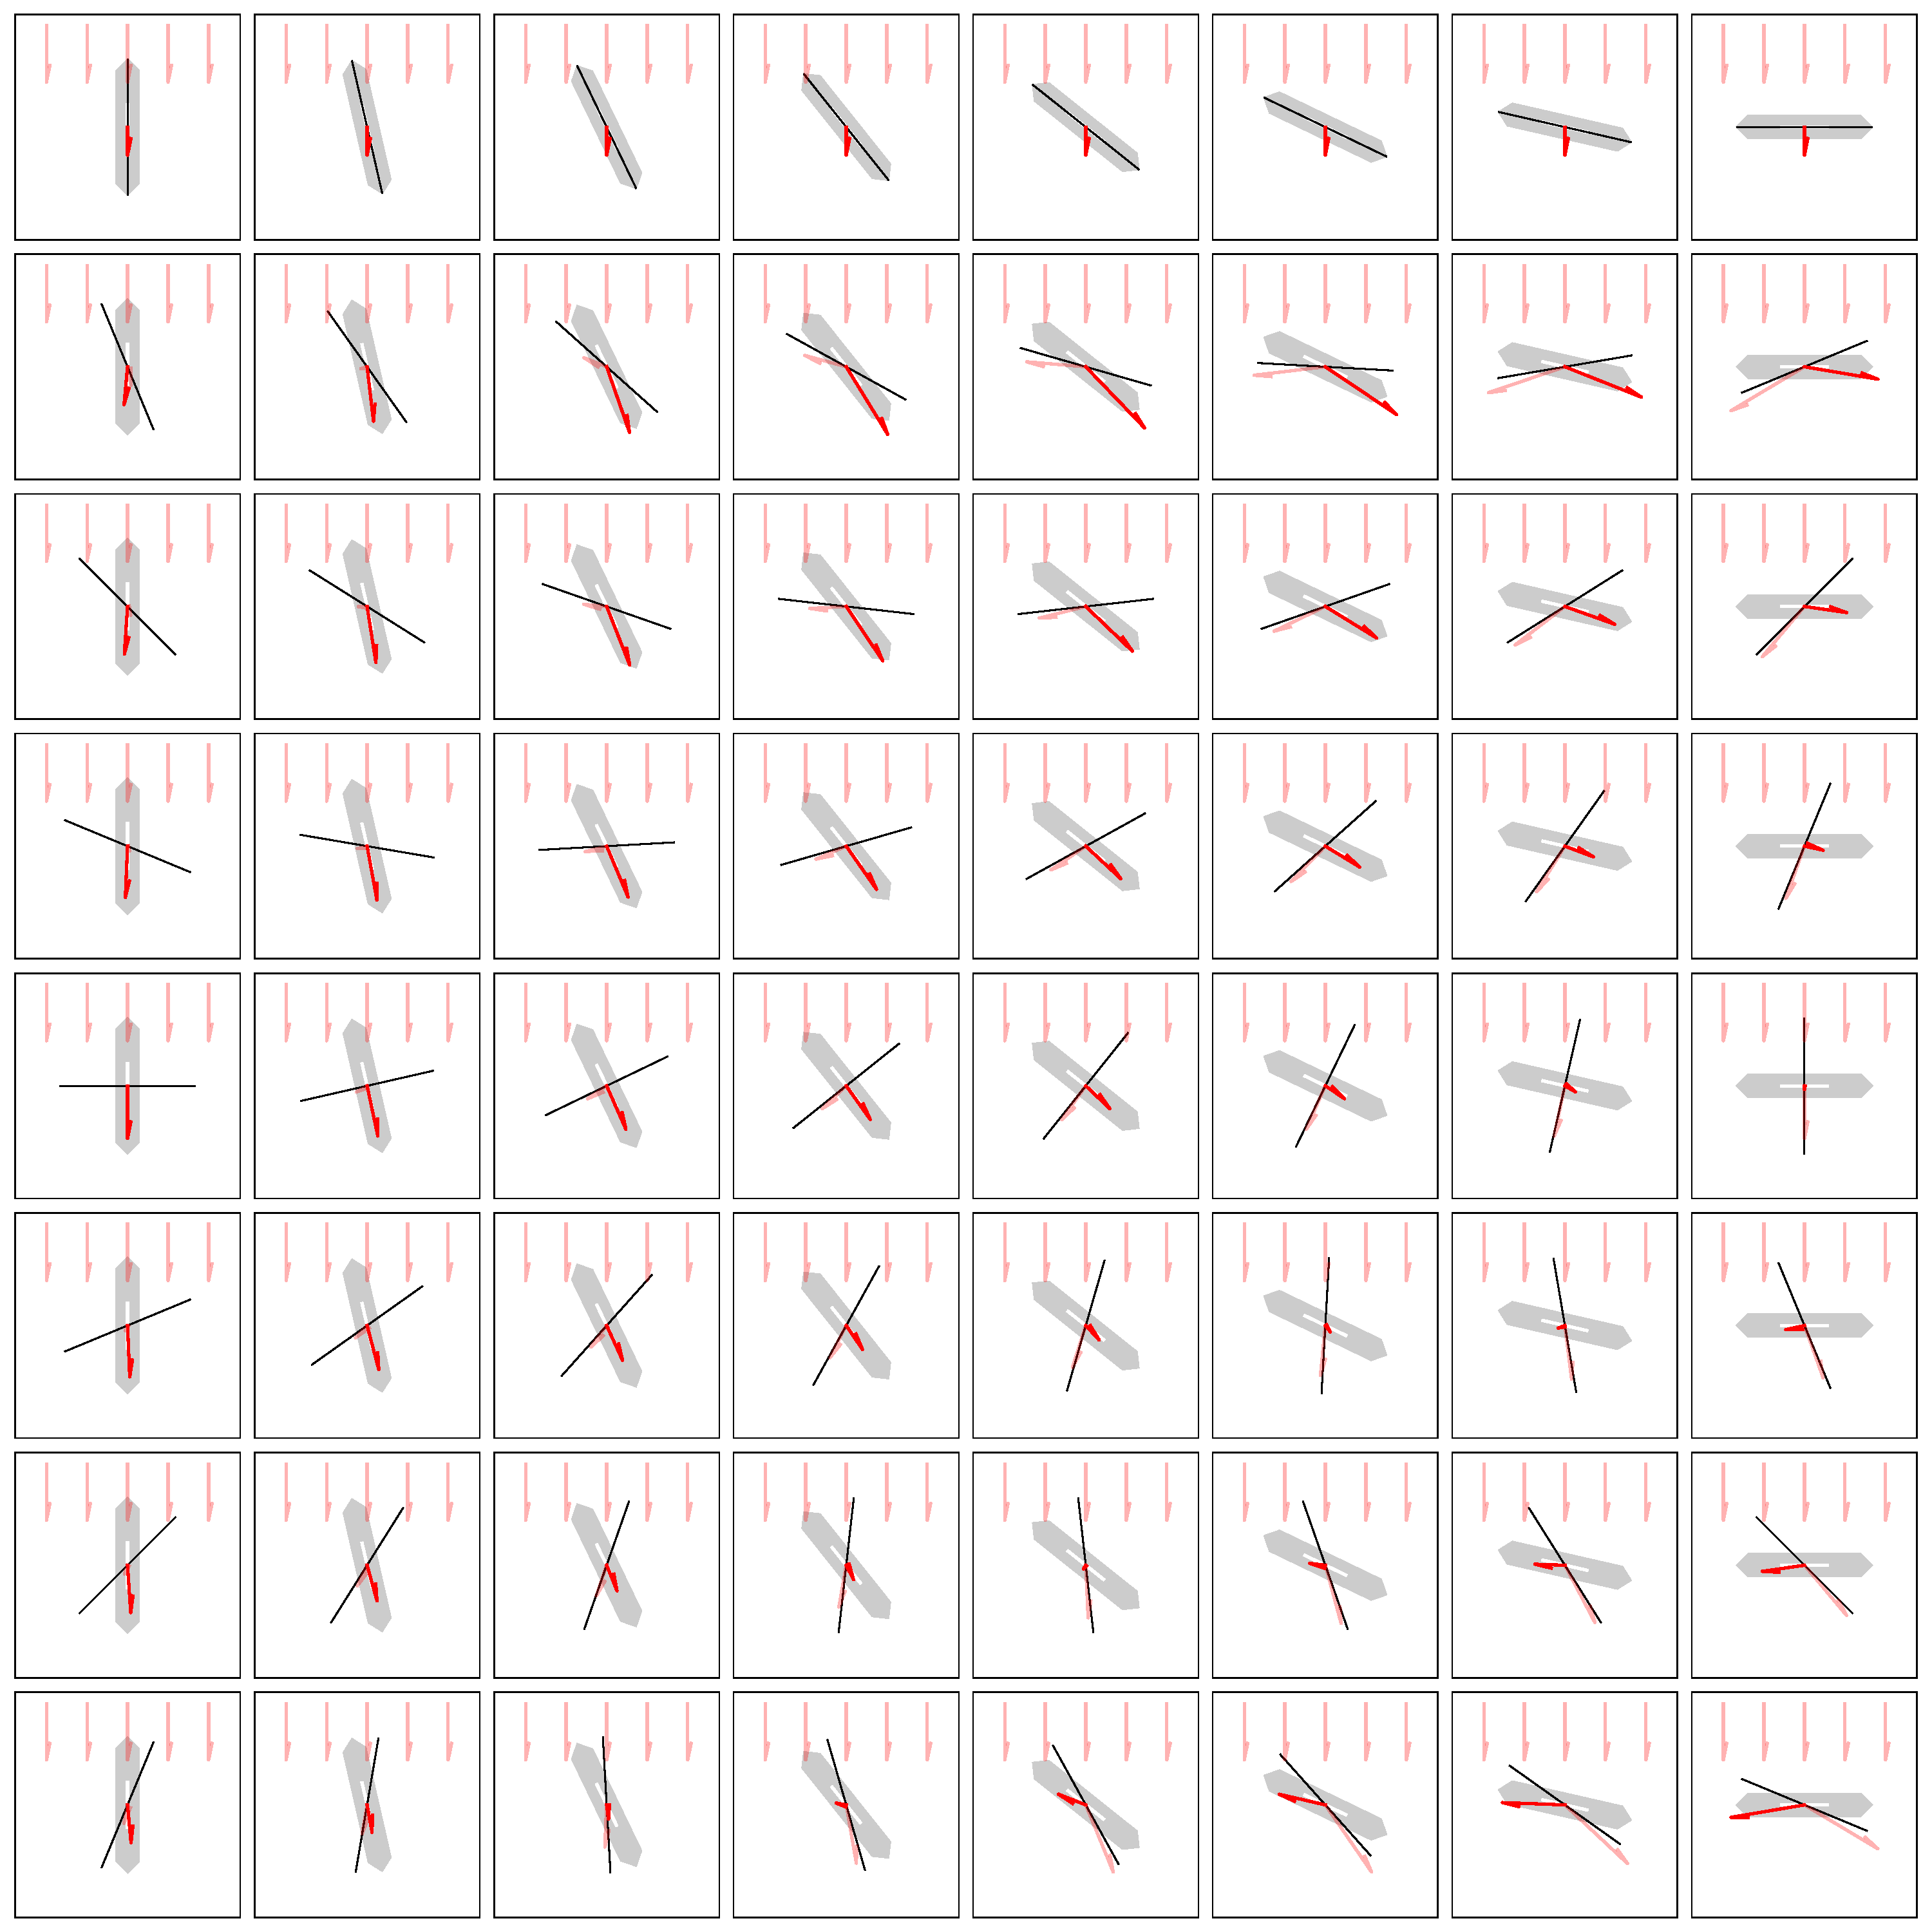
\includegraphics[width=\textwidth]{steady.pdf}
  \caption{Visualizations of the boat velocity $\vboat$ for different settings of the orientations of the keel and sail, all presented in the water rest frame.
  The views are top-down; the keel is represented by a thick grey line, the sail is represented by a thin black line, and the wind and boat velocities are represented by black arrows.
  Most of the settings of the keel and sail lead to downwind travel, but a few in the top-left quarter of this grid lead to upwind travel.\label{fig:steady}}
  \figurerule
\end{figure}

One comment to make is that if you look carefully at the panels of \figref{fig:steady}, you can see that, even in the rest frame of the water, the boat doesn't sail \emph{precisely} in the direction the keel is pointed.
It is close in most cases, but not precisely aligned.
This makes sense, because the wind is always---in some sense---trying to blow the sailboat downwind.

It might seem strange, in \figref{fig:steady}, that the keel orientation is marked but not the direction that the boat (the prow of the boat) is pointing.
Right now, the concept of ``forwards'' and ``backwards'' for the boat is a bit soft.
The boat is defined, in some sense, by the force laws.
These, in turn, are, in some sense, quadrupolar.
So the boat doesn't really have a front and a back!
We will get more serious about deliberately sailing in a particular direction in \secref{sec:good}.

In \figref{fig:hourglass} we show the distribution of relative boat--water velocities one obtains if one randomly orients one's sail and keel.
These orientations are literally randomly chosen angles from the uniform distribution on $[0,2\pi)$.
Many of the resulting boat--water velocities are near zero, because randomly orienting your keel and sail is not a good way to sail!
\begin{figure}[t!]
  ~\hfill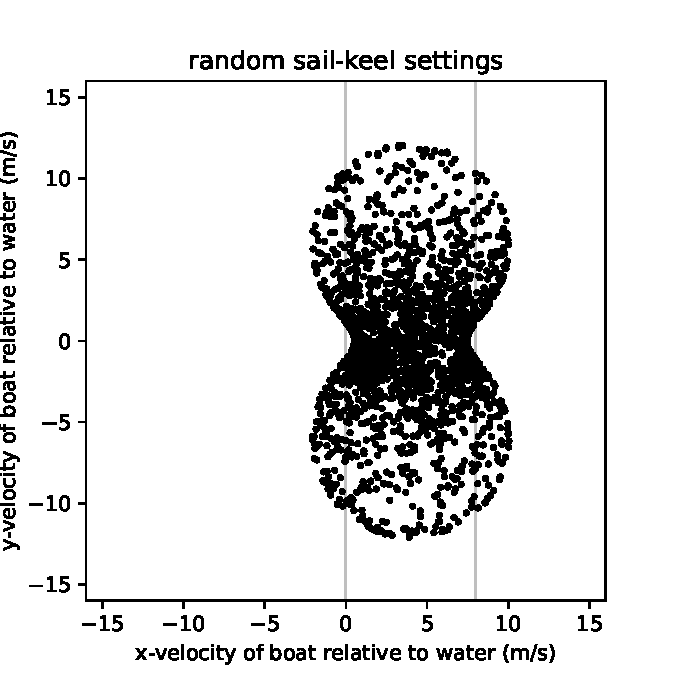
\includegraphics[width=3in]{hourglass-random.pdf}\hfill~
  \caption{The $x$ and $y$ coordinates of the relative boat--water velocity $\vboat-\vwater$ for a set of randomly oriented keels and sails.
  For all of these trials, the relative wind--water velocity is $\vair-\vwater=(8\,\mps)\,\uvec_x$ (that is, $8\,\mps$ in the $x$ direction), as it is in every panel of \figref{fig:steady}.
  Points to the left of the leftmost vertical grey line are sail--keel settings for which the boat sails upwind. Points to the right of the rightmost vertical grey line are sail--keel settings for which the boat sails downwind faster than the wind.
  There are no settings that go \emph{directly} upwind, and no settings that go \emph{directly} downwind faster than the wind.\label{fig:hourglass}}
  \figurerule
\end{figure}

There are many comments to make about the distribution of velocities shown in \figref{fig:hourglass}.
Here are a few:
There are many sail--keel settings that lead to travel at a boat--water velocity magnitude larger than the wind--water velocity magnitude.
You can't make any settings that give the boat precisely zero velocity with respect to the water.
The wind always blows it at least a bit.
There are many sail--keel settings that lead to downwind travel \emph{faster than the wind}.
Not \emph{directly} downwind faster than the wind, but faster than the wind.
That is, a sailboat can beat an air balloon at downwind travel even in stationary water!

There are, of course, many sail--keel settings that lead to upwind travel.
Not \emph{directly} upwind, but upwind.
That makes sense; the whole point (in some sense) of building a model of a sailboat is to understand how it sails upwind.
In \secref{sec:design} we will return to the upwind travel; we will show that in principle you might be able to build a boat that can travel upwind \emph{faster than the wind}.
Indeed, this boat (specs in \secref{sec:design}) does not sail upwind very fast, and it can't sail at an angle that is even close to directly upwind.
This closest angle to directly upwind will also be a function of the design of the boat.

One might ask: Intuitively, how does upwind travel work?
You can think of the boat like a slippery wedge, with the wind pushing on one side of the wedge (the sail) and the water pushing on the other side of the wedge (the keel).
The wedge slips forward.
Maybe that helps?
HOGG SAYS: I THINK WE NEED A DIAGRAM HERE, SHOWING DWFTTW and UW.

Finally, although upwind travel is slow going, with lots of tacking (HOGG DO WE NEED TO DEFINE THIS? YES WE DO) required, if you are situated \emph{on the boat}, upwind travel \emph{feels very fast}.
Why?
Because your experience of speed is, at least in part, the feeling of the wind in your face.
If you think about \figref{fig:hourglass} in terms of the boat-air velocity instead of the boat-water velocity---that is, if you Galilean-boost to the rest frame of the air---the upwind travel has much larger boat-air velocities than the downwind travel.
So even though you can sail fast downwind, it sometimes \emph{feels} faster upwind.

\section{Good sailing}\label{sec:good}

In \secref{sec:steady} we showed how the boat moves (in steady state), given any arbitrary setting of the orientation of the keel and the sail.
However, one doesn't sail by randomly setting the keel and sail!
One sails by pointing the boat in some direction and setting the sail (or sails) appropriately given that boat pointing, or vice versa.
In our simple, ram-pressure boat, how should we set the planar sail?

We could define \emph{GoodSailing(tm)} to be setting the sail orientation optimally, given the orientation of the boat.
This might look something like the following:
\begin{align}\label{eq:good}
    \uvec_{\perp\sail}^\good &\leftarrow \argmax_{\uvec_{\perp\sail}} \left[\uvec_{\parallel\keel}\cdot(\vboat-\vwater)\right] ~,
\end{align}
where $\uvec_{\perp\sail}^\good$ is the best orientation of the (planar) sail conditioned on the orientation of the keel,
$\uvec_{\parallel\keel}$ is the unit vector pointing along the keel (parallel to the keel, in the forwards direction),
the inner product gives the projection of the boat--water velocity vector onto the boat heading direction,
and (for optimization purposes) the velocity difference $\vboat-\vwater$ is implicitly a function of the sail and keel orientations, according to the model of \secref{sec:steady}.
This optimization is one-dimensional, but it is a global optimization, so it requires some attention; details of our implmentation of the optimization are given in \secref{sec:implementation}.
Some examples of GoodSailing(tm) settings of sail and keel are shown in \figref{fig:good}, along with the resulting boat velocity vectors.
A summary of all possible boat--water velocity vectors possible, for GoodSailing(tm) at many different keel orientations, is shown in \figref{fig:hourgood}.
This latter figure is sometimes called a ``speed diagram'' \cite{pos}; it is standard in all books on the subject of sailing (HOGG GIVE REFERENCES and figure numbers).
\begin{figure}[t!]
  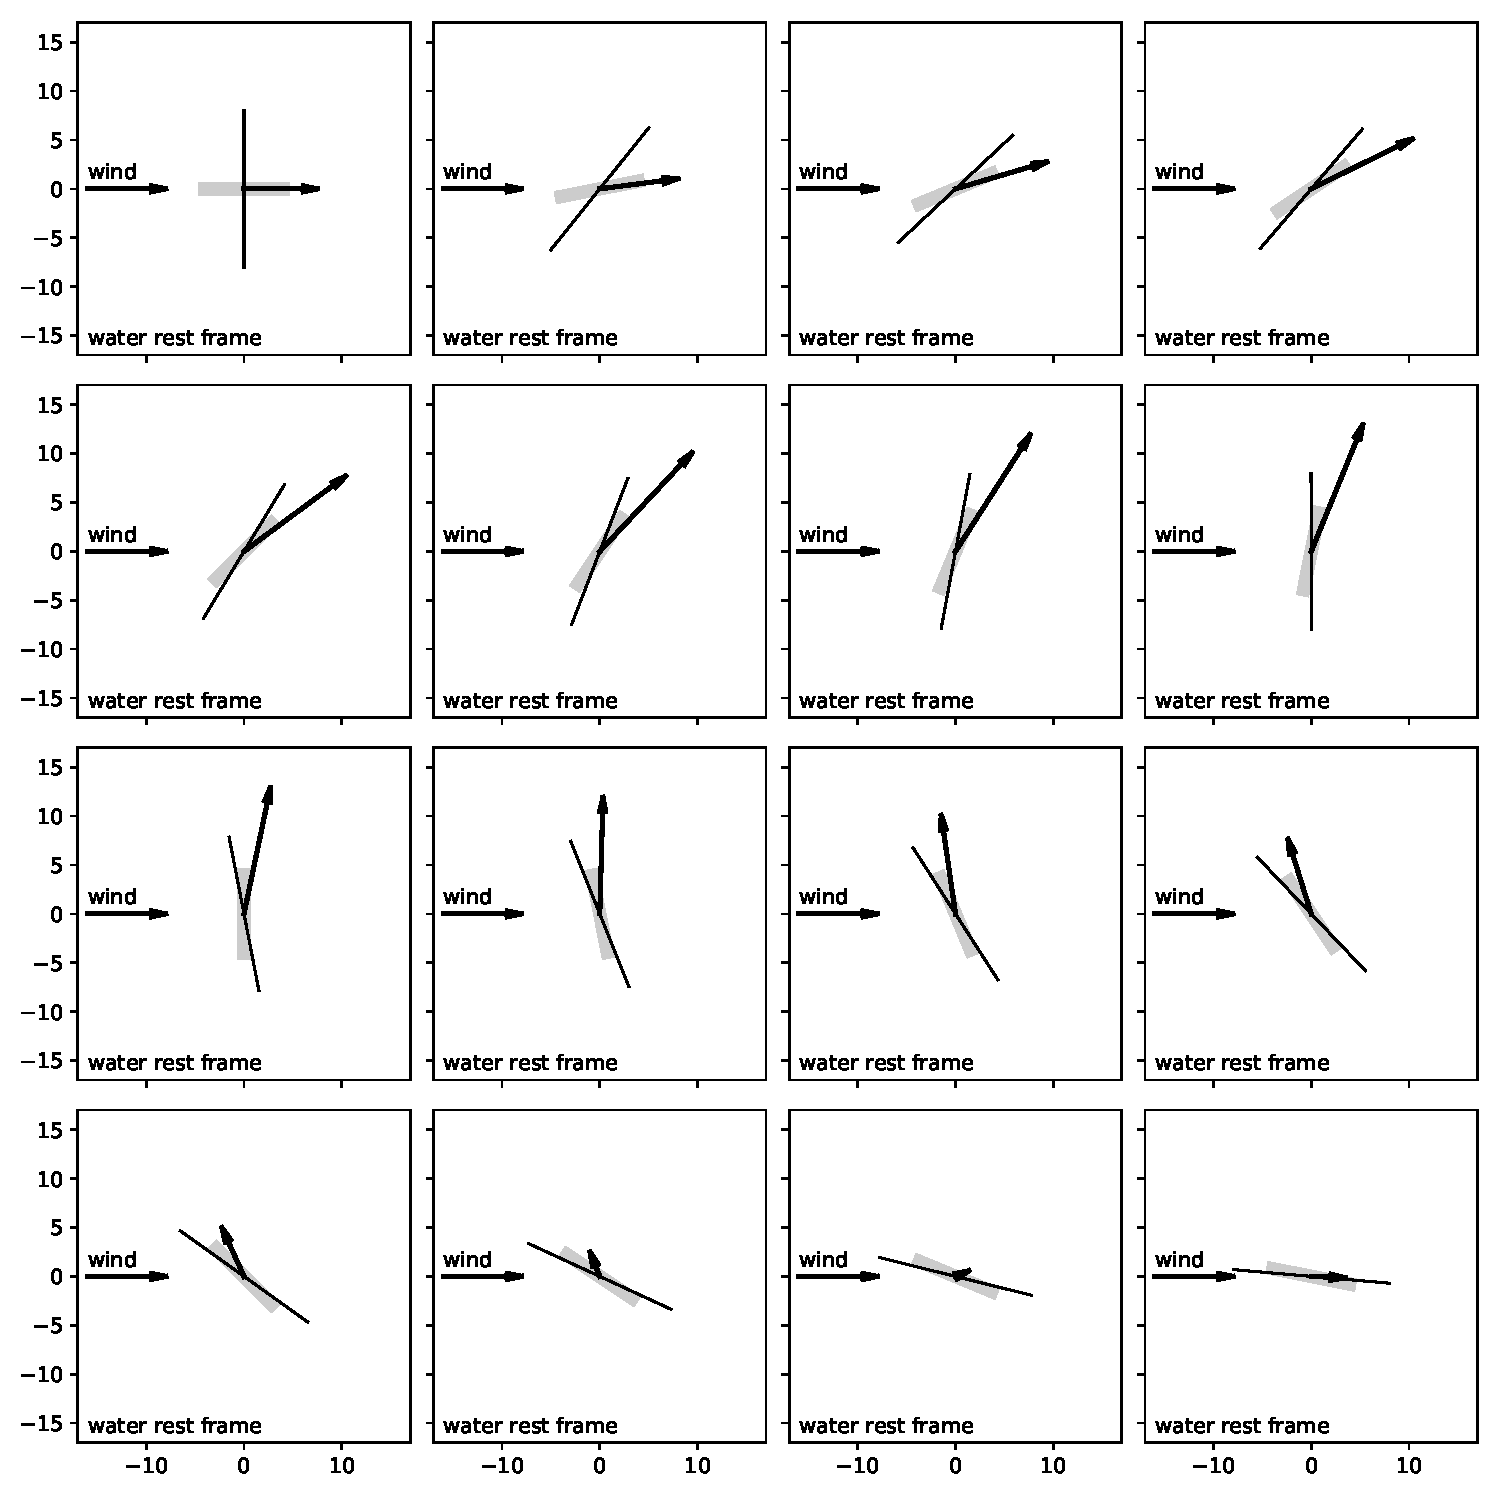
\includegraphics[width=\textwidth]{good.pdf}
  \caption{Visualizations of GoodSailing(tm) for different settings of the orientation of the keel.
  Conventions are the same as in \figref{fig:steady}.
  GoodSailing(tm) is unsuccessful in the last two cases, where the pointing is too close to directly upwind.
  In these cases the the maximum of the GoodSailing(tm) objective \eqref{eq:good} is negative.\label{fig:good}}
  \figurerule
\end{figure}
\begin{figure}[t!]
  ~\hfill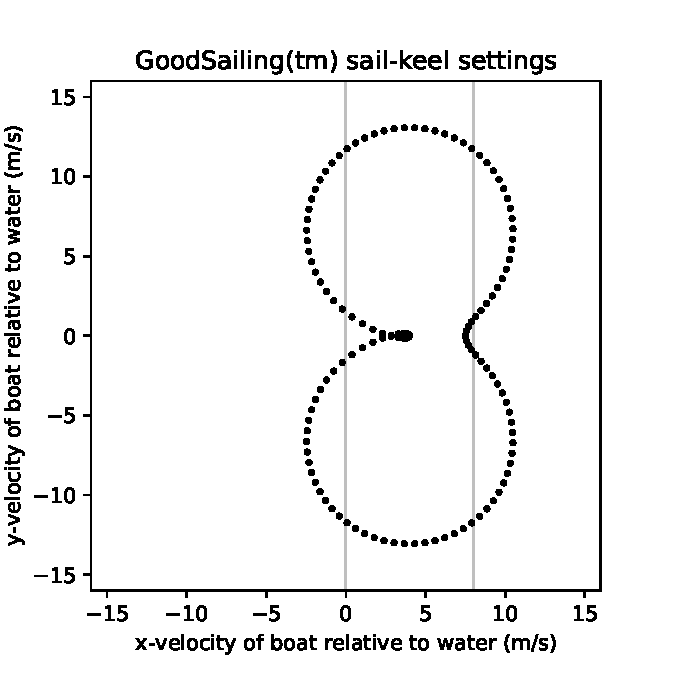
\includegraphics[width=3in]{hourglass-good.pdf}\hfill~
  \caption{The $x$ and $y$ coordinates of the relative boat--water velocity $\vboat-\vwater$ for GoodSailing(tm) for a set keel orientations.
  For all of these trials, the relative wind--water velocity is $\vair-\vwater=(8\,\mps)\,\uvec_x$ (that is, $8\,\mps$ in the $x$ direction), as it is in every panel of \figref{fig:good}.
  Compare this to \figref{fig:hourglass}.
  As is visible in \figref{fig:good}, when the keel orientation is too close to directly upwind, the boat goes downwind instead; there are no \emph{directly} upwind options. This figure is sometimes called a ``speed curve'' \cite{pos}. It is directly comparable to [HOGG WHAT FIGURES IN THE BOOKS ABOUT SAILING?].\label{fig:hourgood}}
  \figurerule
\end{figure}

There are many comments to be made here about GoodSailing(tm), but mainly the point is that GoodSailing(tm) confirms what we saw in \secref{sec:steady}.
You can sail upwind, you can sail faster than the wind, and you can even sail downwind faster than the wind.
You can't sail \emph{directly} upwind, and you can't sail \emph{directly} downwind faster than the wind.
You can't give the boat precisely zero velocity with respect to either the water or the air, and the boat doesn't sail exactly in the direction it is pointed (it sails downwind of that, relative to the water).
In detail, to an experienced sailor, the trim of the sail in \figref{fig:good} might look a little ``tight'' relative to standard best practice.
But of course our sail is a planar approximation to a real sail; the curvature of the sail makes these angles wrong in detail (the angles shown in \figref{fig:good} are not quite right for either the boom or the bulk of any curved sail).
The details of \figref{fig:hourgood} will depend on the physical properties or design of the boat.
We return to this point in \secref{sec:design}.

GoodSailing(tm) is good!
But it is not the \emph{best} a sailor can do, for various reasons:
One is that the boat does not move relative to the water exactly in the $\uvec_{\parallel\keel}$ direction, so the optimization for the projection onto $\uvec_{\parallel\keel}$ might not be quite right.
Another is that the destination might also be moving with respect to the water (for example, if the destination is on the banks of a flowing river), so the relative velocity in \eqref{eq:good} is the wrong relative velocity.
Yet another is that you might have a destination in mind that is directly upwind or directly downwind and you will need to not just optimize your velocity but instead take a non-trivial tacking path.
We address a few of these next.

\section{Better sailing}\label{sec:better}

A type-A sailor---or maybe a competitive sailor---is trying to get from a current position to a destination as quickly as possible.\footnote{%
We don't particularly endorse this attitude towards sailing. The journey \emph{is} the destination.}
Our view is that this sailor should start by specifying the unit vector $\uvec_\destination$ that points from the current position of the boat towards the destination of the boat.
The sailor should then maximize the scalar product of the boat's velocity (relative to the destination) onto the unit vector pointing to the destination.
That is, we could define BetterSailing(tm) as
\begin{align}\label{eq:better}
    \uvec_{\perp\sail}^\better,\uvec_{\perp\keel}^\better &\leftarrow \argmax_{\uvec_{\perp\sail},\uvec_{\perp\keel}} \left[\uvec_\destination\cdot(\vboat-\vdest)\right] ~,
\end{align}
where $\uvec_{\perp\sail}^\better,\uvec_{\perp\keel}^\better$ are the best settings of the orientations of the keel and sail, given the direction $\uvec_\destination$ to the destination, and (because we are Galilean-relativistic) this velocity is relative to the velocity $\vdest$ of the destination (which might not be stationary with respect to the water; imagine that we are sailing on a fast-flowing river).
In this expression \eqref{eq:better}, implicitly $\vboat$ is being thought of as a function of the orientations (and more).
Note that the sailor \emph{does not necessarily want} to travel directly towards the destination:
The sailor wants to make as much progress as possible in that direction, but is willing to tack back-and-forth to get there, if it gets the boat there faster.
So the optimization objective really is the projection of the boat velocity onto the displacement vector pointing from the current position of the boat to the destination.
While this is all simple to state, the global optimization is a bit painful to implement in code.
We give details in \secref{sec:implementation}.

We show examples of BetterSailing(tm) in \figref{fig:better}, where we show the direction to the destination and the settings of the keel and sail.
In these examples, we have set the velocity of the destination equal to the velocity of the water, but this will not be the case in general.
In \figref{fig:hourbetter} we show the velocities obtained in BetterSailing(tm), which are a subset of the velocities obtained in GoodSailing(tm).
In particular, the velocities that are not optimal for some particular destination are not used.
\begin{figure}[t!]
  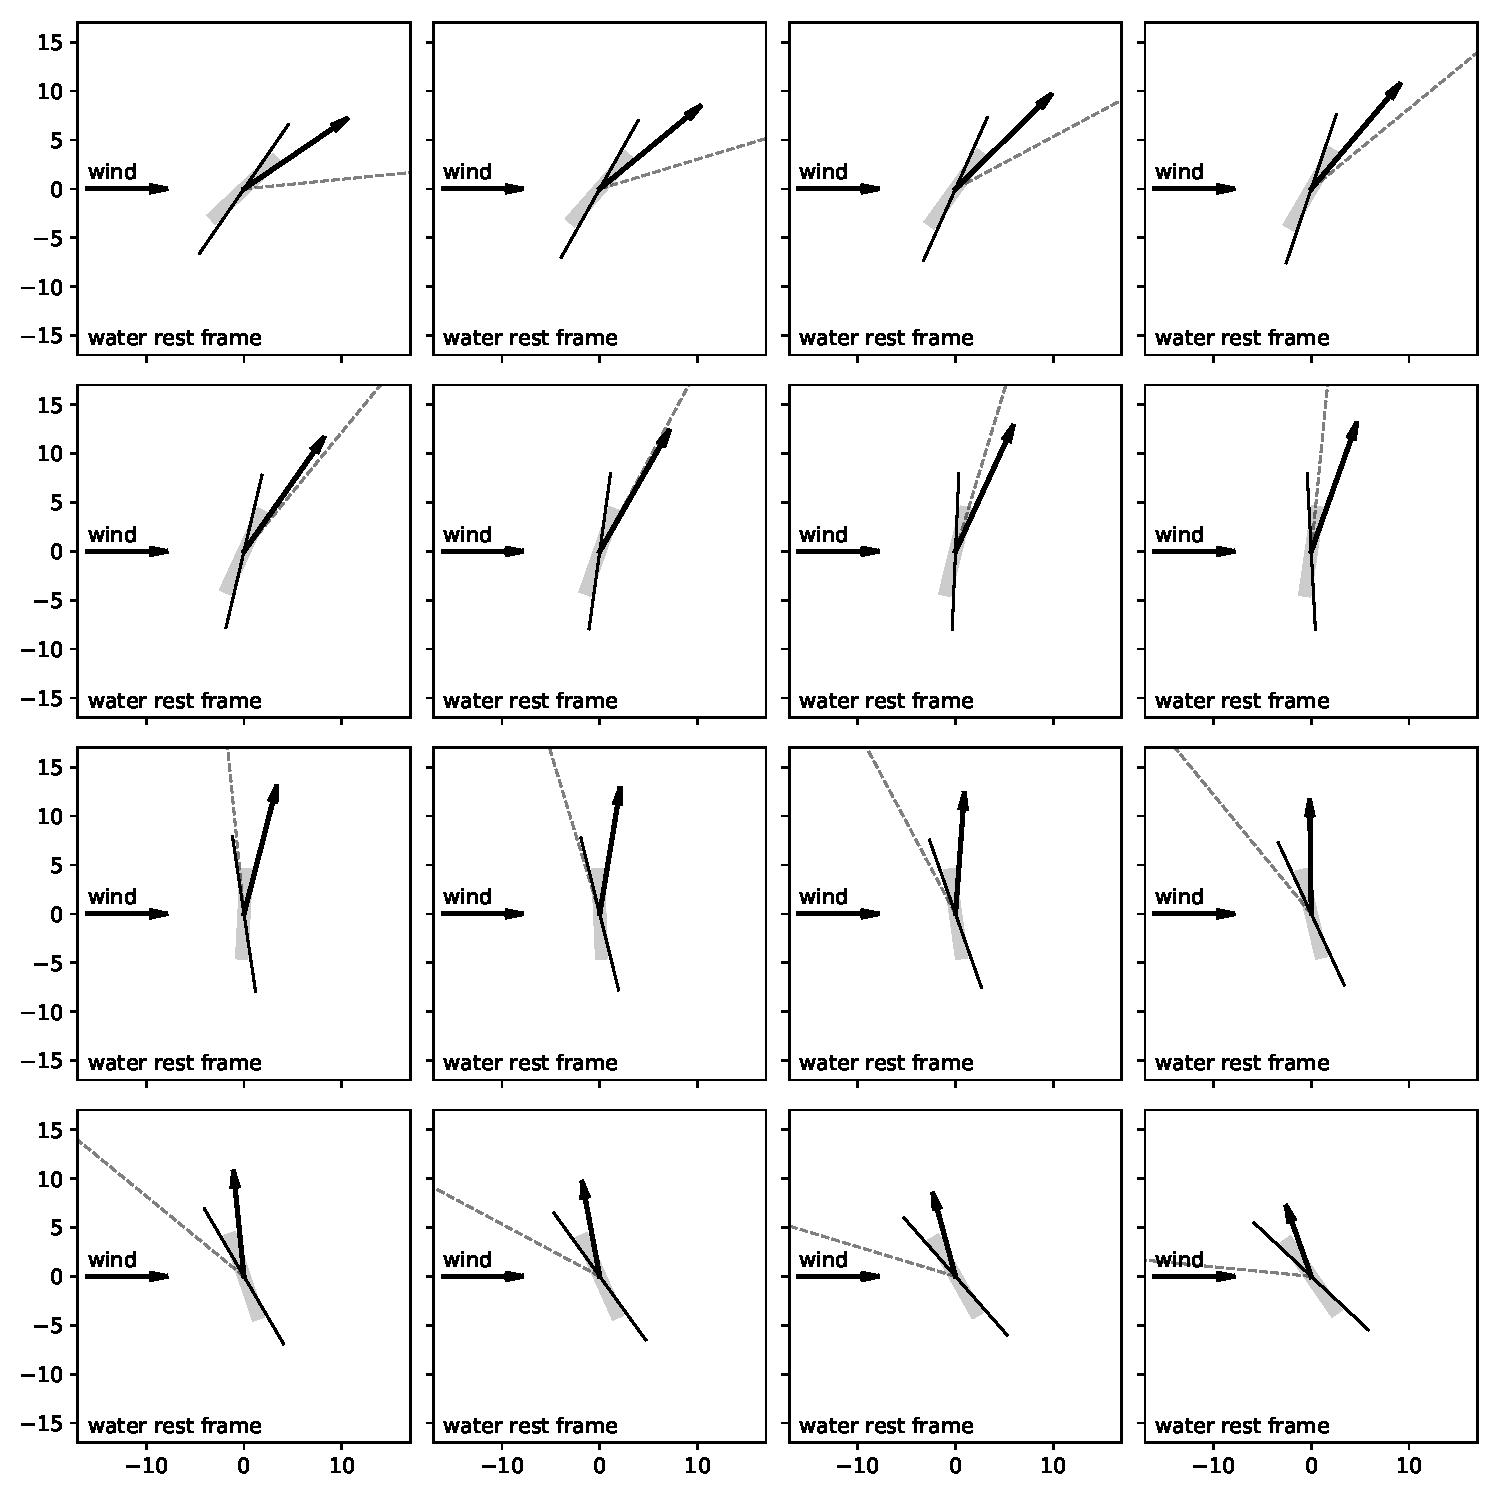
\includegraphics[width=\textwidth]{better.pdf}
  \caption{Visualizations of BetterSailing(tm) for different directions to a distant destination.
  Conventions are the same as in \figref{fig:steady} and \figref{fig:good}, except that now the destination direction is indicated with a dashed path line.
  These plots assume that the destination is stationary with respect to the water ($\vdest-\vwater=\vec{0}$).
  BetterSailing(tm) often involves sailing at a substantial angle to the direct line towards the destination.
  In these cases, the idea is that the best route to the destination involves frequent tacking back and forth across the path to the destination.\label{fig:better}}
  \figurerule
\end{figure}
\begin{figure}[t!]
  ~\hfill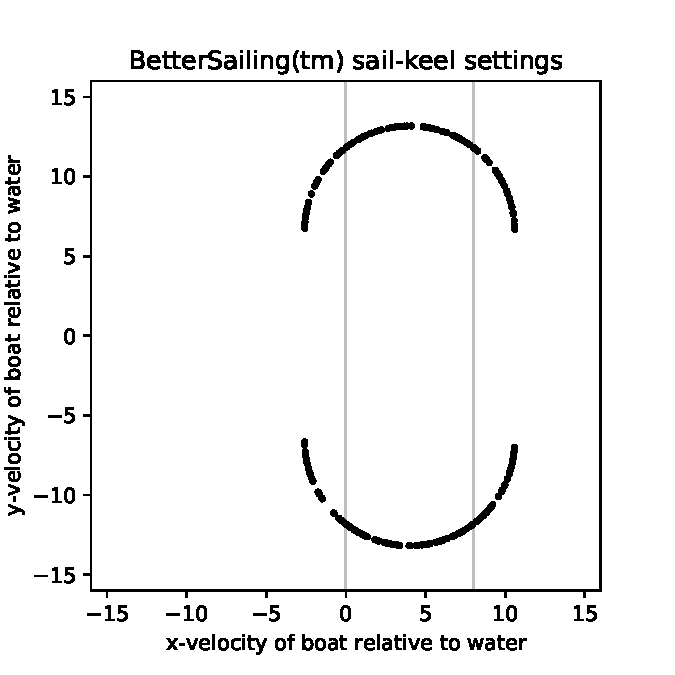
\includegraphics[width=3in]{hourglass-better.pdf}\hfill~
  \caption{The $x$ and $y$ coordinates of the relative boat--water velocity $\vboat-\vwater$ for BetterSailing(tm) for a set of destination vectors of different orientations.
  For all of these trials, the relative wind--water velocity is $\vair-\vwater=(8\,\mps)\,\uvec_x$ (that is, $8\,\mps$ in the $x$ direction), as it is in every panel of \figref{fig:better}.
  Compare this speed curve to \figref{fig:hourglass} and also to \figref{fig:hourgood}.\label{fig:hourbetter}}
  \figurerule
\end{figure}

BetterSailing(tm) is better than GoodSailing(tm), because BetterSailing(tm) takes better account of the sailor's objectives.
However, BetterSailing(tm) is \emph{still} not the best we can do.
For example, a sailor must in general take non-trivial tacking paths from origin to destination (especially when the destination is upwind, but even when the destination is downwind).
The corners of that path---``coming about'' in sailing parlance---cost time, so their frequency should be balanced against slightly non-optimal sailing directions.
Thus an even better sailor will put the boat into configurations that don't appear in \figref{fig:hourbetter}.
The full exposition of this requires a model for the costs of coming about.
That's outside the scope of this \documentname.

\section{Boat properties and boat design}\label{sec:design}

In all of the experiments and figures given above, we made use of a model boat with the following effective areas: HOGG SAY: THESE ARE NOW CONSISTENT WITH THE NOTEBOOK, BUT NOT WITH THE FIGURES. NEED TO PULL IN NEW UPDATED FIGURES.
\begin{align}
  A_\sail / A_\keel &= 700 \quad\mbox{(sail-to-keel ratio)}\label{eq:boat1}\\
  A_\sail / A_\above &= 200 \quad\mbox{(sail lift ratio)}\\
  A_\keel / A_\below &= 200 \quad\mbox{(keel lift ratio)}\label{eq:boat4}
\end{align}
This boat is designed such that $\rho_\air\,A_\sail = \rho_\water\,A_\keel$, which seems sensible, but is perhaps not industry standard.
This boat also has very good drag ratios or lift ratios:
The sail lift ratio (the ratio of effective area of sail to hull-above) is 250, as is the keel lift ratio (the ratio of effective area of keel to hull-below).
All these ratios were set not by analyzing any real boats, but by making the speed curve shown in \figref{fig:hourgood} look reasonable, or accord with expectations set by the books on the physics of sailing HOGG CITE THESE.

In thinking about these areas, recall, for one, that our boat is a brutal approximation!
For two, these areas are \emph{effective areas} within this brutal approximation, not measured areas.
Probably the least realistic of these effective-area ratios is $A_\keel/A_\below$; probably real boats rarely have this keel lift ratio in the hundreds.
In this sense, maybe our model is more appropriate for an ice yacht than a sailboat?
HOGG BUT SEE THE AMERICA'S CUP BOATS!

HOGG NOW ADDRESS THE EXCELLENT LIFT RATIOS.

As we change the ratios of the effective areas, the shapes of the velocity curves change.
In \figref{fig:design} we show the effect on the boat velocity curves of changing the ratios $A_\sail/A_\keel$, $A_\sail/A_\above$ (the sail lift ratio), and $A_\keel/A_\below$ (the keel lift ratio)....HOGG
\begin{figure}[t!]
  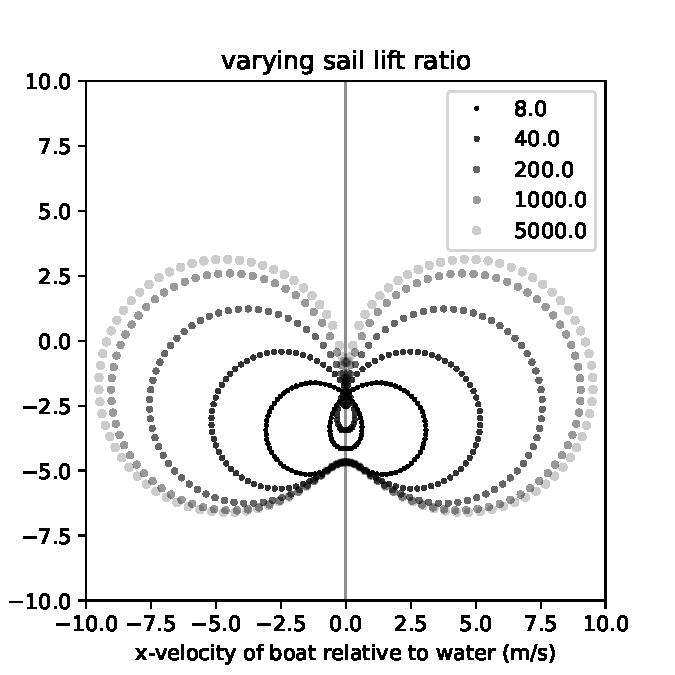
\includegraphics[width=0.5\textwidth]{design_A.pdf}%
  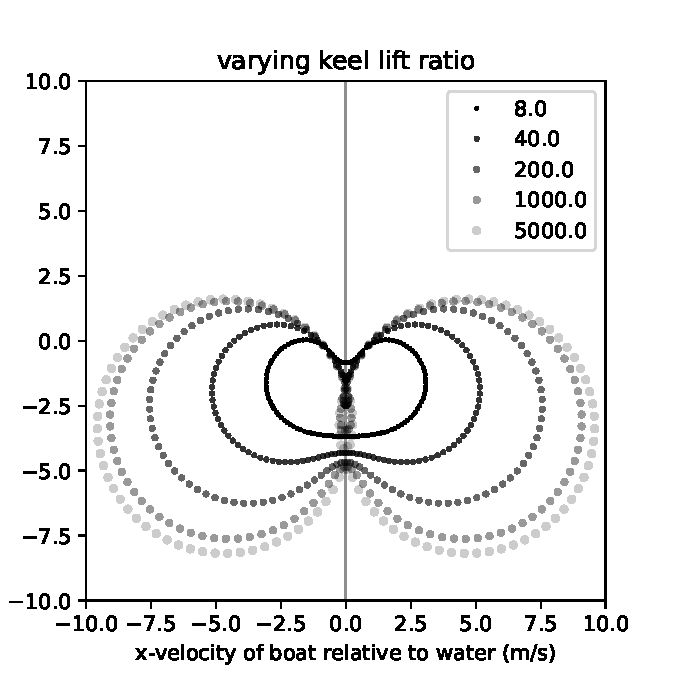
\includegraphics[width=0.5\textwidth]{design_C.pdf}\\%
  ~\hfill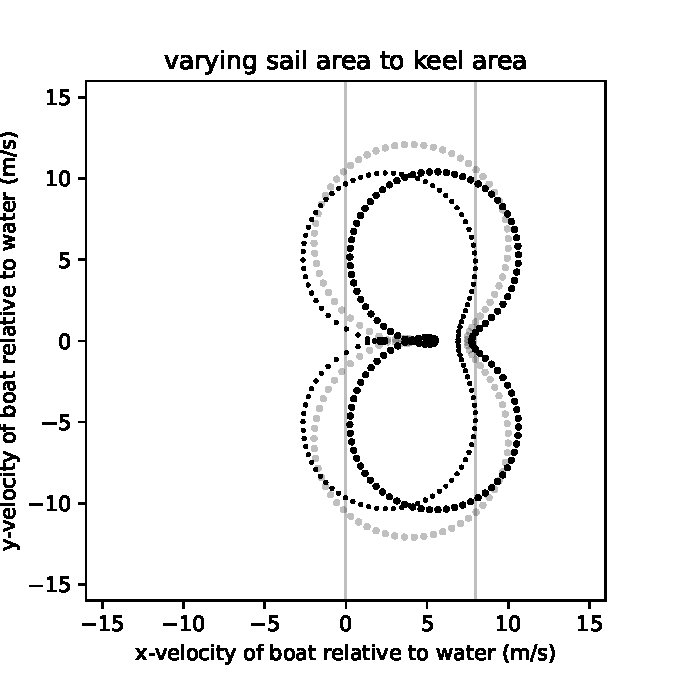
\includegraphics[width=0.5\textwidth]{design_E.pdf}\hfill~
  \caption{Each panel is analagous to \figref{fig:hourgood} but in each case we have varied one of the boat's dimensionless ratios. In each panel, the grey points show the same speed curve as that plotted in \figref{fig:hourgood}, which was computed for the boat described by the parameters given in \eqref{eq:boat1} through \eqref{eq:boat4}, and for a wind speed (relative to the water) of $8\,\mps$.
  In the top-left panel, the small and large black points show variations as we vary the sail lift ratio $A_\sail/A_\above$ from 40 (small dots) to 200 (grey dots) to 1000 (large dots).
  In the top-right panel, the small and large black dots show variations as we vary the keel lift ratio $A_\keel/A_\below$ from 40 (small dots) to 200 (grey dots) to 1000 (large dots).
  In the bottom-left panel, the small and large black dots show the variations as we vary the sail-to-keel ratio $A_\sail/A_\keel$ from 140 (small dots) to 700 (grey dots) to 3500 (large dots).\label{fig:design}}
  \figurerule
\end{figure}

HOGG: Comment on what we see in \figref{fig:design}. HOGG: Note that if you set $\rho_\air\,A_\sail=\rho_\water\,A_\keel$ you get the fastest possible cross-wind sailing speed. Is that a result, and is it known?

HOGG maybe take the limit of infinite lift ratios and show that you get absurd results.

HOGG: 
A true boat has sails that are globally curved,\footnote{%
In the local-curvature or Riemann-curvature senses, sails are often not (very) curved; after all, they are often made from flat pieces of fabric.
However, they are curved in the global or colloquial sense: Different patches of the sail have differently oriented normal vectors.
It is in this colloquial sense that we are using the words ``curved'' and ``flat''.
All that said, the most sophisticated sails in the world are also curved in the local sense \cite{sails}.}
and forces that are different in detail from these pure ram-pressure forces.
HOGG: REPHRASE: The curvature of the sails will in general rotate the air force vectors towards the direction in which the boat is pointed.

HOGG: make sure we consistently use the term ``lift ratio'' for the air and the water, and that this is a real term.

\section{Numerical implementation notes}\label{sec:implementation}

HOGG: Newton's method (CITE), invert, solve, etc.
Note that in practice, Newton's method works amazingly well.
For Newton's method we make use of the derivatives---HOGG GIVE HERE THE DERIVATIVES of the ram-pressure expressions---which are order-2 tensors.

HOGG: How we implement GoodSailing(tm) and BetterSailing(tm) optimizations. It's a mess!

\section{Discussion}\label{sec:discussion}

This \documentname{} presented what we believe to be the simplest model of sailing that is both physically realizable and also reproduces most of the salient features of the behavior of sailboats.
The model is simple to state, makes use of nothing more than undergraduate mechanics, conforms to Galilean relativity and coordinate freedom, and is extremely easy to implement numerically.
It makes explicit that the boat is powered by the relative velocity of the air and water.
It demonstrates that it is easy for a sailboat to travel faster than the wind (or, to be specific, to travel relative to the water faster than the magnitude of the relative wind-water velocity).
It demonstrates that there is nothing physically strange about being able to travel, by sailboat, upwind, or downwind faster than the wind, in both cases by taking a tacking course.
Along the way, we found that the best sail-to-keel effective-area ratio for cross-wind sailing is the ratio of the density of water to the density of air; and we found that keels ought to be curved like sails (HOGG DO WE EXPLICITLY DISCUSS THIS ABOVE? IF NOT, WE SHOULD, WHERE WE DISCUSS THE SYMMETRY BETWEEN SAIL AND KEEL, OR WHERE WE DISCUSS THE CURVATURE OF THE SAILS.)
For both of these ``predictions'' there seems to be evidence in the designs of the best-in-class sailing vessels today.

This model makes brutal assumptions and approximations.
In some sense, this is the ``spherical cow'' model of a sailboat.
It literally assumed (incorrectly) that the hull of the boat is spatially isotropic (cylindrically symmetric).
It assumed that viscosities are negligible, and that the effects of turbulence are all perfectly captured by a trivial ram-pressure expression (force proportional to an area times velocity squared).
The model assumed that the drag coefficients $\eta$ do not depend on the angles of the sail or keel, nor on the relative speeds of air, water, and boat.
The model ignored that the wind is gusty, and that wind speeds (and water speeds), in the real world, vary with height (and depth).
All these approximations are wrong in detail.
They could be fixed and accuracy could be improved, but at the expense of adding many new parameters and constants, which distract from the principal story:
Sailing is a very simple phenomenon from a fundamental-physics perspective.

HOGG: This is a momentum-transport model! NOW Take some time to bash the Bernoulli bullshit. Note also that the different-path-length part of that argument is explicitly not true for a sail!

HOGG: Speaking of misconceptions: These results probably do indeed show that you can travel directly downwind faster than the wind. That maybe resolves some folk conflicts or arguments?

HOGG: This model implies, indirectly, that keels should be curved! And they are, in high-end sailing (HOGG cite?)

We expressed pride that our model is explicitly Galilean-relativistic.
That begs the question: What about special relativity?
Of course our model is consistent with special relativity; Galilean relativity is the low-velocity limit, when all relative velocities have magnitudes way less than the speed of light.
Now what about \emph{relativistic sailing?}
Because we have such a simple model, we conjecture that there might be a version for a star ship that sails by photon pressure (or on stellar winds or supernovae ejecta or other quasi-relativistic flows).
Most contemporary thinking about solar sails and reflected-photon propulsion is thinking in terms of sailing purely ``down wind'' of a single, nearby star, which dominates the photon pressure on any active surface.
But the Galaxy is filled with stars!
With multiple sources of illumination, in principle one might be able to make a photon-pressure vehicle that can sail or tack in arbitrary directions, given illumination from multiple stars.
This might involve a relativistic generalization of the above.
HOGG: Someone must have thought of all this before! CITE THEM.

We defined GoodSailing(tm), which is an optimal setting of the orientation of the sail, given the orientation of the boat.
And we defined BetterSailing(tm), which is an optimal setting of both the orientation of the boat and the orientation of the sail, given the direction to the destination.
But even this is not the best you can do, because optimal sailing (from a time-to-destination perspective) involves complete path planning, constrained to start at the origin and end at the destination.
For destinations that are close to directly downwind or directly upwind of the origin, this complete path planning will involve tacking the boat.
Each tack involves a ``coming about'' or a rotation of the boat to put the wind on the other beam (HOGG CORRECT LANGUAGE HERE?).
Each coming about costs time.
So optimal path planning must involve that cost, factored against the requirement (if you delay coming about) that you will sail beyond the limits of what BetterSailing(tm) recommends, given your destination.
That is, the global optimal path will not be locally optimal at all points.
A full discussion of this path planning is out of scope for this \documentname, but clearly interesting from an engineering perspective.

HOGG: All code used to make the figures in this \documentname{} are available HOGG WHERE?

\paragraph{Acknowledgements:}
It is a pleasure to thank Will Kinney (Buffalo), Hans-Walter Rix (MPIA), Hyung-Don Ryoo (NYU), and Soledad Villar (JHU) for valuable discussions and comments.

% \raggedright
\bibliographystyle{hogg-plain-annote}
\bibliography{sailing.bib}
% \printbibliography
\end{document}
